\documentclass[12pt, draft]{article}

\usepackage{graphicx}
\usepackage{comment}
\usepackage{float}
\usepackage{hyperref}
\usepackage[authoryear]{natbib}
\usepackage{setspace}
\usepackage{mathtools}
%\usepackage{aas_macros}
\usepackage{amssymb}
\usepackage{textcomp}
\usepackage{siunitx}

\title{Acousto-Optical Tunable Filter Atmospheric Imager for Determination of Aerosol Extinction}

\author{Brenden J Elash, Adam E Bourassa, Douglas A Degenstein, Paul(?)}

\begin{document}
\renewcommand\bibname{BiBTex.bib}

\maketitle

\section{Introduction}

The Atmospheric Limb Imager (ALI) is a prototype atmospheric instrument developed at the University of Saskatchewan with the eventual plan for a satellite instrumentation in the future with the purpose to gather high resolution horizontal and vertical aerosol extinction profiles. The purpose of the ALI prototype is to test and verify the use of an Acousto-Optical Tunable Filter (AOTF), the fundamental technology behind ALI, in a space environment and to be gather atmospheric sulfate aerosol profiles with high spacial resolution. ALI will measure light from the atmosphere through the limb geometry which measures the radiance from scattered sunlight from the sunlit atmosphere. ALI is a single channel instrument measuring radiance from the visible to the near infrared wavelengths (650-950~nm) and through successive images build spectral information. The system uses a telescoptic front end to pass collimated light through through the AOTF which is then focused onto the the detector. The AOTF has the unique property of separating the incoming radiance into each of its polarized components selecting one and rotating it polarization through 90 \si{\degree} allowing on to recover some polarization information of the incoming radiance. The ALI prototype was complete in August of 2014 with a stratospheric balloon test flight from the Canadian Space Agency balloon launch facility in Timmins Ontario onboard the CNES gondola platform on September 20, 2014.

The atmosphere has been monitored in several geometries throughout the history. Occultation was one of the first methods used on satellite instrumentation to measure atmospheric quantities including ozone which included SAM II \citep{McCormick1979}, SAGE II \citep{McCormick1987}, and SAGE III \citep{Thomason2003}. Different instrumentation using other geometries were also put into space to acquire atmospheric data for different species with altering resolutions and the quantity of data that could be acquired in a single day. One such geometries is the limb geometry which measures radiance from the sun light atmosphere as it scatters and interacts with molecules in the atmosphere. However, the limb scatter geometry has a complexity that requires a foreword model to be able to model the scattering interaction, both single and multiple, between different consituents in order to be able to acquire any useful atmospheric information form the recorded data. Two instruments from the previous generation of space remote sensing instruments use have sucessfully used limb scatter to determine atmospheric parameters, Optical Spectrograph and InfraRed Imaging System (OSIRIS) an Canadian instrument onboard the Odin satellite \citep{Llewellyn2004} and SCanning Imaging Absorption spectroMeter for Atmospheric CHartographY (SCIAMACHY) onboard the ENVISAT \citep{Bovensmann1999} which are grating spectrometers that can only acquire data at a single altitude at a time so a series of exposures is required to create a vertical profile. The new proposed method with ALI allows for a two dimensional spacial images of a single wavelength polarized light to be acquired giving both vertical and horizontal resolution of the environment through the use of the innovative AOTF technology.

Sulfuric aerosol is a fundamental portion of the global climate balance, work by \cite{Andreae2005} has show that global warming has not been as drastic as perviously expected due to the high amounts of aerosol in the stratosphere currently due to the high volcanic activity. Aerosol is a spherical partial that scattered incoming radiance away from the surface of the planet causing a cooling effect which is dependant on \citep{Kiehl1993}. This effect is fully define by aerosol microphysics requiring accurate knowledge of concentration and particle size distributions. Furthermore, high resolution aerosol measurements are required in order to determine the high extinction area in the atmosphere due to the long path length and high amount of attenuation due to aerosol scattering. Aerosol transportation between across the tropopause are not well known, recently after the 2011 eruption of Nabro it was determined that the asian monsoon has the ability to penetrate through the thermal boundary and eject aerosol from Nabro into the stratosphere \citep{Bourassa2012c}. Current generation instrumentation does not have the necessary resolution needed for current scientific needs and additional horizontal and along the track resolution will allow the determine of aerosol loading from volcanic an anthropogenic sources and as as an losses from the stratosphere that will result in an overall heating of the planet's surface. ALI, a prototype for a next generation of instruments will address the much needed horizontal resolution improvement to help answer the questions about global climate.

In this paper the first section will outline the technology behind the AOTF used within the ALI system and then describe the optical design behind ALI and an ulterior optical presentation including and comparison with the Belgium instrument ALTIUS. Followed by ALI's maiden flight onboard the CNES CARMEN gondola from the CSA balloon launch facility in Timmins, Ontario including the conditions and trajectory of the flight day, and the measurement taken during the campaign including an analysis of the conversion from raw measurement into calibrated data. Lastly, an retrieval algorithm for aerosol extinction and particle size parameters will be outlined and then preformed on the from the data for the campaign.

\section{Instrument Design}

\subsection{Acouto-Optical Tunable Filter}

n order for the AOTF to allow the filtering of a specific wavelength a momentum matching criteria must be held where the wave vectors of the acoustic wave match the difference of the incoming and diffracted light wave vectors. This condition is described by
\begin{equation}
    \ \mathbf{k}_{i} = \boldsymbol\kappa + \mathbf{k}_{d}
    \label{eqn:3.1:phaseMatching}
\end{equation}
where $\mathbf{k}_{i}$ and $\mathbf{k}_{d}$ are the wave vectors for the incoming and diffracted light and $\boldsymbol\kappa$ is the acoustic wave vector. These wave vectors can be described by
\begin{equation}
    \ k_{i} = \frac{2\pi n_{i}}{\lambda}
    \label{eqn:3.1:incomingWavevector}
\end{equation}
\begin{equation}
    \ k_{d} = \frac{2\pi n_{d}}{\lambda}
    \label{eqn:3.1:diffractedWavevector}
\end{equation}
\begin{equation}
    \ \kappa = \frac{2\pi F}{\nu}
    \label{eqn:3.1:acousticWavevector}
\end{equation}
where $n_{i}$ and $n_{d}$ are the indices of refraction of incoming and diffracted light. Finally $\lambda$ is the wavelength of light in a vacuum. It will be assumed that the extraordinary light is undergoes the momentum matching through the device. This causes the above refractive indices defined above to be
\begin{equation}
    \ n_{i} = \left( \frac{\sin^{2}(\theta_{i}+\alpha)}{n_{e}^{2}} + \frac{\cos^{2}(\theta_{i}+\alpha)}{n_{o}^{2}} \right)^{-\frac{1}{2}}
    \label{eqn:3.1:incomingIndexOfRefraction}
\end{equation}
\begin{equation}
    \ n_{d} = n_{o}
    \label{eqn:3.1:diffractedIndexOfRefraction}
\end{equation}
where $n_{e}$ and $n_{o}$ are the indices of refraction for the extraordinary and ordinary polarizations of the incoming light and $\alpha$ is the cut angle relative to the piezoelectric transducer and the optical axis. For a crystal, like TeO$_{2}$, the difference in the index of refraction is small and can be approximated as \citep{Voloshinov2007}
 \begin{equation}
    \ n_{i} = n_{o} + \Delta n\sin^{2}(\theta_{i}+\alpha)
    \label{eqn:3.1:incomingIndexOfRefractionApprox}
\end{equation}
where $\Delta n$ is the difference between the extraordinary and ordinary indices of refraction (ie $\Delta n = n_{e} - n_{o}$). The wave vectors, seen in \autoref{fig:3.1:ATOFWavevectors}, of the system need to follow the momentum matching criteria from \autoref{eqn:3.1:phaseMatching}. Separating the wave vectors into their directional components with respect to the cut angle, $\alpha$, the tangential and perpendicular directions respectively are
\begin{equation}
    \ k_{i}\cos\theta_{i} = {k}_{d}\cos\theta_{d}
    \label{eqn:3.1:wavevectorsTangentalDirection}
\end{equation}
\begin{equation}
    \ k_{i}\sin\theta_{i} + \kappa = {k}_{d}\sin\theta_{d}
    \label{eqn:3.1:wavevectorsPerepndicularDirection}
\end{equation}

The tangential direction of the wave vector does not give any helpful information however the wavelength and RF relation can be determined by the perpendicular component of the wave vector by combining \autoref{eqn:3.1:wavevectorsPerepndicularDirection} and the vector diagram seen in \autoref{fig:3.1:ATOFWavevectors} to get
\begin{equation}
    \lambda  = \frac{\nu}{F}[n_{i}\sin\theta_{i}-(n_{o}^{2}-n_{i}^{2}\cos_{2}\theta_{i})^{1/2}]
    \label{eqn:3.1:initialAOTFWavelengthDependance}
\end{equation}

It should be noted that for the geometry defined the incident angle is the same as the Bragg angle. The above can be written as

\begin{equation}
    \lambda  = \frac{\Delta n\nu}{F}\frac{\sin^{2}(\theta_{i}+\alpha)}{\sin\theta_{i}}
    \label{eqn:3.1:AOTFWavelengthDependance}
\end{equation}
assuming difference in indices of refraction is small and the Taylor expansion approximation of the square root is used \citep{Voloshinov2006}. Also, through the described interaction the diffracted light goes though a 90\si{\degree} rotation in polarization \citep{Voloshinov1996}. Lastly, a wide aperture is required for an AOTF used for imaging purposes. These devices have been developed \citep{Gass1991} and are currently readily available for imaging purposes.

Images were taken at a set of RFs spaced every 150 kHz from 160~MHz to 75~MHz and the spectral images were recorded with the spectrometer slit at 0.5~mm making the minimum FWHM of the spectrometer 1.175~nm, which is well below the minimum FWHM of the AOTF listed specifications at 1.6~nm. For each trial at each RF two images were taken with a 15~second integration time: one taken with the AOTF on at a given RF and one with the ATOF off. The stray light entering spectrometer as well as the any dark current and the DC bias are recorded in the image with the AOTF off and can be removed from the AOTF spectral image by taking the image with the AOTF on and subtracting the image recorded with the AOTF off. Then all of the rows of the CCD are summed together to get the total count measurement at each wavelength. The maximum value of each image is taken to be the diffracted wavelength through the AOTF at each respective RF. A typical spectral measurement result can be seen in the top left panel of \autoref{fig:3.1:AOTFCharaterization}. The characteristic sinc function filtering can be seen in the image. Typically the fringes of the sinc function accounts for 16\% of the total signal.

The maximum values from each of the images were determined as well as the wavelength these values occur. It was noted that the curve appear to follow a power function of the form
\begin{equation}
    \ F = a\lambda^{b}.
    \label{eqn:3.1:powerFunction}
\end{equation}
A linear least squares fit was preformed in log space finding the coefficients $a$ and $b$. The fit was performed and appeared to match the data quite well but a relative error analysis was preformed and it was seen that there was a only an agreement better than 0.6\%. A better fit was desired to characterize the AOTF's RF-spectral dependance so a modified power function was used in the form of
 \begin{equation}
    \ F = a\lambda^{b+c\log\lambda}
    \label{eqn:3.1:modifiedPowerFunction}
\end{equation}
or a quadratic least squares fit. These results can be seen in the bottom half of \autoref{fig:3.1:AOTFCharaterization}. The agreement of this form is less than 0.1\% throughout the whole wavelength range and the determined RF and wavelength relation can be seen in
\begin{equation}
    \ F = \exp{19.793}\lambda^{-3.381+0.168\log\lambda}.
    \label{eqn:3.1:modifiedPowerFunctionCoeffiecicents}
\end{equation}
It should be noted that even though the AOTF optical range is 600~nm to 1200~nm this analysis only measures wavelengths from 600~nm to 950~nm. The low quantum efficiency of the CCD and the low NIR emitted from the light source causes wavelengths past this point to be noisy. Thus these measurements were left out and an InGaAs array with better quantum efficiency in the NIR has been acquired and will be used to characterize the rest of the spectral range of the AOTF.

The same set of data was used to determine the FWHM for each of the above determined wavelengths. the results of this study are shown in the top right of \autoref{fig:3.1:AOTFCharaterization}. Wavelengths past approximately 1080~nm are to noisy too be able to determine the FWHM of the signal and will be determined at a later date with the InGaAs Array. However, the AOTF spectral resolution is well within the limits that are required in order to determine aerosol extinction and cloud occurrence in the UTLS.

The diffraction efficiency was also determined for a few points across the wavelength range of the AOTF and the wavelengths results were all within 56$\%$ to 64$\%$ as were stated by the factory specification of the device. Two limb imaging systems have been prototyped for use with the AOTF and their characteristics including advantages and problems will discussed in the following sections.

\subsection{Optical Design and Performances}

TELECENTRIC:

A telecentric layout in both image and object space has an advantage for the imaging quality of the AOTF system shown in \autoref{fig:3.2:telecentricRayTracing}. Since the wavelength filtered by the AOTF is dependant on the incident angle, and from \autoref{fig:3.2:telecentricRayTracing}, all the lines of sight enter with approximately the same angular spread so the filtered image has consistent wavelength. However, two problems are added to the system. First, a blurring effect is added to the final image dependant on wavelength, which will be discussed below in greater detail. As well, this method is sensitive to any surface defects of the crystal since the light enters the crystal in focused bundles.

The overall design has several aspects that make it a good system for imaging. First all of the bundles of light entering the AOTF have the same angular spread. As seen in equation \autoref{eqn:3.1:AOTFWavelengthDependance} the diffracted wavelength depends on the incoming angle or its spread, in this set up all points of the imaging plane will have the same angular dependance so the entire image will be of the same wavelength and have the same spectral bandpass.

%Also, since the system is telecentric, perspective is not a major factor in the final image of the system as an object of same size but at different distances will appear to be the same size in the recorded image.

However, despite its benefits there are a few drawbacks to consider in the design as well. First, the optical path between the two 100~mm focal length lens is 200~mm in air, however the AOTF is made of TeO$_{2}$  or paratellurite and has a high index of refraction of 2.43 and 2.27 for the extraordinary and ordinary optical axis respectively. The crystal also has a high dispersive property, or Abbe number, so the index of refraction depends on the wavelength. The change is distance in the optical path, $d$, is given by
\begin{equation}
    \ d = \frac{n(\lambda)-1}{n(\lambda)}t
    \label{eqn:3.2:opticalPathDisplacement}
\end{equation}
where $n(\lambda)$ is the index of refraction with a wavelength dependance and $t$ is the thickness of the crystal. The AOTF crystal causes the optical path in air to be lengthened by $d$, as can be seen in \autoref{fig:3.2:opticalPathDisplacement}. In order to compensate, the length $d$ must be added to the path to account to the discrepancy, but this can only be accounted for a specific wavelength and thus image defocusing will occur at the image plane for other wavelengths. The severity of this problem can be seen in \autoref{fig:3.2:telecentricSpotSize} from a Code V simulation of the spot size of the optical system . In this simulation a grid of rays is passed through the system for each field of view and using ray tracing the final locations on the image plane are determined. The black circles represent the Airy disks, which are the minimum possible spot size possible limited by diffraction for each wavelength of light. The above analysis was preformed when the system was focused at 800~nm. The spot sizes at 800~nm are on the order of 24~\si{\micro\meter} at the center, which is diffraction limited, and 94~\si{\micro\meter} at the edge of the field of view. However, for the same optical layout the 600\,nm spot sizes are all greater than 160~\si{\micro\meter} which will cause an noticeable blurring in the recorded image.

TELESCOPIC:

The AOTF now has collimated light passing though the device, unlike the telecentric system, and this has a few fundamental changes to alter to the system's imaging quality. First, the primary light passing through the AOTF from a single line of sight is entering the AOTF at the same angle, so the image will have a smaller FWHM than the telecentric counterpart however each line of sight will be diffracted with a different fundamental wavelength due to the angular dependance in the AOTF Bragg diffraction wavelength determination equation (\autoref{eqn:3.1:AOTFWavelengthDependance}). The final image has a smaller spectral bandpass but there will a wavelength gradient radiating out from the center of the image. Second, since the light now passes through the AOTF collimated, the focal point of the image no longer changes with wavelength. Instead a lateral displacement of each line of sight occurs based on the angle of incidence and the diffracted wavelength which causes a slight magnification of the image. The lateral displacement that occurs is given by the following relation
\begin{equation}
    \ \delta = (n(\lambda)-1)\frac{t\theta}{n(\lambda)}
    \label{eqn:3.2:planeParallelDiplacement}
\end{equation}
where $\delta$ is the displacement from the original path; causing a slight magnification change based on the wavelength of the light being diffracted, but this magnification is a negligible change overall, the effect can be seen in \autoref{fig:3.2:planeParallelDiplacement}. The last change to the system is the focusing power it possesses, as can be seen in the spot diagrams in \autoref{fig:3.2:telescopicSpotSize}. The change in spot size due to wavelength is primarily due to the chromatic aberrations of the optical lens. One option is to replace the lenses with mirrors in the flight version which will eliminate the chromatic abberation issue. Second, the system is diffraction limited for 600\,nm for all lines of sight and at 800\,nm at 3.0 degrees. Also the difference in location of the spot sizes is caused by the magnification effect discussed above.

CHOICE:

A final selection for the optical design of ALI will be presented in this section as well the justifications used to determine the result. Furthermore, a comparison with the prototype Belgium instrument will be made to demonstrate the differences between the two instruments. For the final design of ALI the telescopic system deemed to be the better option for our scientific purpose to determine aerosol extinction and engineering study to verify the capabilities of using an AOTF in space based remote sensing techniques.

The telescopic system offers the ability of having an image plane location that is not dependant of the wavelength being imaged leading to a system that would either require the system to have mechanical pieces to move the imaging plane or additional optical components to counter act the change in the optical path. Using mechanic components to move the camera would be an addition failure point and would have to be well calibrated across the whole wavelength range. For the other alternative a custom lens or prism would need to be created in order to counteract the defocusing effect of the AOTF which would cause further reflections within the system increasing the possibility of stray light hitting the CCD camera and well at decreasing the signal through put of the system. This design also allow for a greater focus on spacial resolution that could be achieved with a telescopic system with is necessary in order to be able to image the fine structure of aerosol concentration on the order of 100s of metres.

Another minor consideration for the system is the finer FWHM for each line of sight that passes through the ATOF and is imaged on the CCD giving more fine spectral resolution however the draw back is that the central wavelength of each line of sight is dependant upon the angle of incident. A wavelength gradient appears in the final image in the the longest central wavelength occurs in the center of the image and radiates outward towards shorter wavelengths as apparent in \autoref{eqn:3.1:AOTFWavelengthDependance} an have a wavelength gradient of approximately 7~nm at 650~nm central wavelength and 11~nm at 950~nm, however for a space based instrument with a relatively smaller field of view the gradient could be reduced to as small as 2~nm across the whole image with, at worse, the same size as the FWHM of the AOTF. The effect would be a significant problem for instruments measuring trace gasses absorbtion lines, for example water vapour, but aerosol is a broadband enhancing feature in which its effect are visible in atmospheric measurement from 400~nm well into the IR. The wavelength dependant magnification mentioned earlier only amounts to being a change of a approximately 4 pixels in both direction from the inherent magnification from 650~nm to 950~nm overall this change is considered negligible for the purpose of ali's mission which will be discussed in \autoref{sec??}.

The final optical specification for ALI can be found in \autoref{tab:3.2:ALISystemParameters}. A noticeable change from the telescopic prototype is the decreased f/\# and the front end demagnification and the back end magnification which have all were all related to increasing the signal entering ALI. The lower F/\# increases the amount of light that can enter the optical chain allowing for shorter exposure time that were needed in order to get high quality data from the Timmins, Ontario campaign. The increase F/\# required larger optics and has as such a larger beam of light to pass into the AOTF, which unfortunately was not possible due to the AOTF having a fixed aperture of 10 by 10~mm. To rectify this problem a found end demagnification was added to reduce the size of the incoming light beam entering he AOTF down to a size that could pass through its optical aperture and remagnify it back to its original size with the back end optics before passing into the imaging system. Lastly, the specifications for the wavelength range was decreased from 600-1200~nm down to 650-950~nm, which was done for two different reason at each end of the spectrum. At the 600~nm side of the range the effeminacy of the optical components antireflection coasting started to fall and the AOTF itself diffraction efficiency fall off quickly at wavelengths lowers than 630~nm. These loss in efficiencies would require large integration times during flight that would not have been practical so they were removed from the instruments range, and even 650~nm has exposure time on the longer side of reasonable. At the long wavelengths the system was originally have a beam splitter to have the image focused on an InGa array for the NIR and a CCD for the visible region which was to be implemented when a folded mirror optical system was to be implemented, but the launch date for ALI was pushed up by one year and no longer gave the time required to design the folded optical system so a linear lenses non-beam spitted system was to be used in stead. The inherent nature of the change of date made it a requirement to reduce upper limit of ALI's wavelength range to 950~nm instead of the originally proposed 1200~nm.

\begin{table}[!ht]
    \begin{center}
    \begin{tabular}{|l|c|}
      \hline
      Effective focal length (mm) & 74.3 \\
      \hline
      Front optics magnification & 0.67 \\
      \hline
      Back optics magnification & 1.27 \\
      \hline
      Field of view (\si{\degree}) & 6.0 x 6.0 \\
      \hline
      F-number & 7.5 \\
      \hline
      Image Size (mm) & 9x9\\
      \hline
      Spectral Range (nm) & 650-950\\
      \hline
    \end{tabular}
    \end{center}
    \caption{ALI Final System Optical Parameters.}
    \label{tab:3.2:ALISystemParameters}
\end{table}

 ALTIUS, a Belgium instrument, uses similar technology as ALI except uses a telecentric optical layout and is designed to measure atmospheric trace gases \citep{Dekemper2012}. Trace gases have narrow absorbtion to emission features that require specific wavelength knowledge. A telecentric layout will give a of constant wavelength across the whole field of view to be able to be able to resolve absorbtion features. The optical specifications are similar between the two instruments, however two key differences will be noted. First, the field of view of ALTIUS is smaller at 5.73x5.73\si{\degree} and if ALI would have used a telecentric design then it would have had an identical field of view due to the geometry and optical requirements of the telecentric layout. In a telecentric design the AOTF aperture directly limits your instruments field of view and both system use an ATOF crystal with an optical aperture of 10x10~mm. Second, the f-number for ALTIUS is 14.32 compared to ALI's 7.5 which allows ALI to increase light throughput at the cost of higher abberations in the final image.

\section{Stratospheric Balloon Flight}

\subsection{Flight Day Conditions and Flight Path}

At the balloon launch base in Timmins, Ontario is located at 48 29.08728~N 81 18.08094~W and ALI at the base on Auguest 28, 2014 with a launch window from September 8 to 14, 2014. In between arrival and launch ALI needed to be integrated onto the CARMEN gondola and verify no conflict or problems with CARMEN's system, including communications. ALI was orientated so it would be 90\si{\degree} with an over heading of a southern field of view during the mission.

The flight of CARMEN was delayed due to poor weather conditions during the launch window. On September 20, 2014 at 05:35 UTC (01:35 local time) ALI was launched for the Nimbus 7 mission onboard the CNES CARMEN gondola from the Canadian Space Agency Timmins Balloon launch base. During the launch the evening was clear with light wind allowing for an safe and ideal launch. The ascent of CARMEN occurred in darkness and reached its flight altitude of 36.5~km at 8:17 UTC. First light was observed by ALI at 9:39 UTC and recorded measurements until 14:42 UTC when the primary aerosol mission was completed. Until ALI power off at 17:15 UTC ALI recorded measurement for secondary goals, including an azmuth scan. A visualization of the flight path with all major landmarks noted can be found on \autoref{fig:5.1:nimbus7FlightPath}.

During the mission a operational mode for aerosol was ran that gathered images from 650-950~nm with 25~nm separation approximately every 25~s. A unique feature of the AOTF is that the diffraction can be disabled to take an image with the filter disabled. These so called 'dark images' allows capture of the stray light in post processing without having any signal in the image allowing for an accurate method of removing stray light.

\subsection{Measurements}

The inherent nature of a AOTF based instrument results in only a specific polarization of radiance being measured by the device. The AOTF measures light entering the AOTF vertical from the front face of the AOTF in the factory specified orientation. Transferred to the orientation of the crystal inside the ALI instrument and direction mounted on the gondola, ALI measured light that is polarized 90\si{\degree} from the horizon or what will be known as the vertical polarization. This results in a system where ALI only measures 10 to 35 \% of the incoming radiance and required a model that can compute polarization in order to successfully use the data from ALI.

The raw flight (level 0) data must be converted to relative radiances (level 1 data) before they can be used to retrieve aerosol extinctions and particle sizes. The transformation includes removal of dark current, the DC bias, stray light removal, and flat fielding. Using the dark images from the assent of the flight combined with laboratory dark test images a table of value based on exposure time and CCD temperature was determined to be able to remove the DC bias and dark current from each raw image. Once completed, the constant offset caused by the DC bias allows for the rest of the analysis to be preformed in counts per second, by taking the counts in the image and divided by the exposure time, in order to easily relate the radiance of different image directly to each other without having to scale the results with respect to the exposure time.

Stray light removal has always been a difficult in atmospheric instrumentation due to the difficulty in accurately discern the strong signal in regard to the relatively weaker stray light signal. Furthermore, an optical system has the further addition of unwanted light thought the rejection of one of the polarizations due to the nature of the AOTF. The signal enters the optical system unpolarized, but the AOTF only operates on one polarization. The entering light is passed through a linear polarizer with an extinction ratio of at least 100,000:1 extinction ratio to remove the unwanted polarization however a small percentage still makes it through the system adding additional stray light. The active filtering of the AOTF allows for an image to be measured where the filtering device is disabled allowing only the stray light to be captured by the measurement, and during ALI's aerosol mode a 'dark image' was captured before every image with the active filtering enabled. By removing the 'dark images' from the signal-stray light contaminated images the end result is image that only contain the measured signal. The previous method was tested in the lab with a known source with even illumination across the field of view of the system, the resulting final image is left with a even decrease in intensity radiating from the center of the field of view as it expected with the know vignetting of ALI.

All that was left to transform the images into usable level 1 data is to add a flat fielding coefficients across the systems spectral and spacial field of view. To determine the flat field coefficient ALI was set up when a quartz-tungsten halogen bulb that is passed through a diffusing plate to give a even laminar radiance across the entire field of view of ALI. Several series of measurement were taken at wavelengths the same as ALI's aerosol mode and used to normalized the full field of view of ALI across the whole spectrum to the center off the 750~nm images, given a relative calibration of radiance referenced to this point. The process used to determine the flat fielding coefficients started with similar process used to remove the stray light during the flat fielding images. Then the images had the DC bias and dark current removed for proper unbiased comparisons and converted to counts per second. Each value of every pixel in the active region of the CCD was normalized to the mean of the value on the center 10 by 10 pixels at 750~nm over all exposure times and trials. The coefficients for flat fielding can be determine to make the radiance value across all field of views and wavelengths relatively calibrated. These coefficients are then applied to the data from the flight that give relative radiances for each pixel. And create a 2D image with resolution of 22 by 22 arcseconds which can be seen in TODO:createfgure.

To increase the precision of the measurements from the flight the images were averaged in 25 horizontal and 10 vertical columns decreasing the resolution to 9.2 by 3.7 arcminutes but greatly reduced the error on the results. A large number of vertical profile with a horizontal dependance could be determined from the new radiance vectors. The final results with error bars can be seen in TODO:makefigure.

\subsection{Retrievals}

The modeled radiance were computed with the SASKTRAN radiative transfer for for High Resolution (SASKTRAN-HR) measurements using the newly developed polarization module. The model uses given atmospheric states to solve the radiative transfer equation to determine the final radiance. SASKTRAN-HR solves the single scatter equation that follows \begin{equation}
    I(s_{1}) = I(s_{0})e^{-\tau(s_{0}, s_{1})}+\int^{s_{1}}_{s_{0}}k(s)J(s)e^{-\tau(s, s_{1})}ds
\end{equation}
where $I(s_{1})$ is the final radiance after scattering though the path from $s_{0}$ to $s_{1}$, the first contribution to the final radiance is the attenuated light from the sun to the observer at $s_{1}$. The second term takes the source term, which is the radiance scattered into the line of sight $J(s)$, and ingrates line of sight with attenuation to determine the scattering contribution to the final radiances. The extinction given by $k(s)$ is the sum of the number density, $n(s)$, time the cross section , $\sigma(s)$ over all species. The polarized output of SASKTRAN-HR gives the stokes vectors for the radiance on its internal coordinate grid which can be retrieved from the model and then can be rotated to match the ALI's coordinate system.

The relative radiance level 1 data from ALI are used create a measurement vector, $y$, from the data seen in the following
\begin{equation}
    \mathbf{y} = \frac{I(\mathbf{z},\lambda)}{I(z_{ref},\lambda)}-\frac{I_{rayliegh}(\mathbf{z},\lambda)}{I_{rayliegh}(z_{ref},\lambda)}
    \label{eqn:measurementVector}
\end{equation}
where $I(z,\lambda)$ is the measured radiance from ALI and $I(z_{ref},\lambda)$ is a reference altitude used to normalize the signal from a high altitude were there is little aerosol contribution, for ALI the highest possible altitude where ALI still as usable signal is around 26-30~km tangent height which brings out the aerosol signal in the vector. The second term is modeled values from SASKTRAN-HR with polarization and only background atmosphere to remove the rayleigh background form the measured radiances which is done to improve the convergence of the retrieval. A base aerosol state or a priori, $\mathbf{x}$, for aerosol extinction profile is used in the SASKTRAN-HR model and give the foreword model seen below that is used in the Multiplicative Algebraic Reconstruction Technique (MART).
\begin{equation}
    \mathbf{F}(\mathbf{x}) = \frac{I_{mod}(
    \mathbf{z},\lambda)}{I_{mod}(z_{ref},\lambda)}-\frac{I_{rayliegh}(\mathbf{z},\lambda)}{I_{rayliegh}(z_{ref},\lambda)}
    \label{eqn:forewordModel}
\end{equation}
where $I_{mod}(z,\lambda)$ is the modeled radiance for the measurement and $I_{mod}(z_{ref},\lambda)$ is the measurement at the same reference altitude for normalization. The foreword model is in combination with the measurement vector is updated using the MART algorithm
\begin{equation}
    x_{i+1} = x_{x}\sum_{j}\frac{y_{j}}{F(z_{j})}W_{ij}
\end{equation}
where $i$ is the aerosol extinction at each measurement altitude and $j$ is the tangent point internal to the SASTRAN Model. $W_{ij}$ is the weighting matrix that relates the tangent altitudes to the measurement altitudes. This method was outlined by \cite{Degenstein2009} and allows for fast retrievals with calculating a Jacobian.

Once the retrieval has been preformed for a series of wavelengths a determination for the angstrom exponent occurs. Since the measurements observe relatively the same atmosphere over the time of one complete aerosol cycle. The differences between extinction ratio at the different wavelength can be used to gather a understanding of aerosol particle size in the form
\begin{equation}
    \frac{n\sigma}{n_{0}\sigma_{0}} = \left(\frac{\lambda}{\lambda_{0}}\right)^{-\alpha}
    \label{eqn:agstromCoefficient}
\end{equation}
where $n$ is the aerosol concentration, $\sigma$ is the cross section, and $\alpha$ is the angstrom exponent. Since the cross section of aerosol is dependant on not only the wavelength but also the partial size and distribution the angstrom coefficients give information of particle size. For the retrieval described here a single mode log-normal distribution is assumed with a mode radius, $r_{g}$, and the mode width, $\sigma_{g}$ which is commonly used \citep{Bingen2004}. At each altitude the extinction from each wavelength is used to fit a line and determine the angstrom coefficient for every altitude. Then the median value from altitudes is used as the new size parameters in SASKTRAN with the mode width set at a constant 1.6 an the mode radius is varied to achieve an identical angstrom coefficient determined. Then the MART algorithms is rerun to update the aerosol extinctions and then the angstrom coefficients are found again and the process goes through several iterations. At the end of the last iteration the angstrom coefficient profile is kept unaltered as the final product.

\subsection{Results}

What the final measurements showed and how they compare to SOLAMON and OSIRIS

\section{Conclusions and Future Prospects}

Self explanatory.

Figures for Measurement and retrieval section not completed yet.

\newpage
\bibliographystyle{thesis}
\bibliography{BiBTex}

\newpage

\begin{figure}[h!]
    \begin{center}
    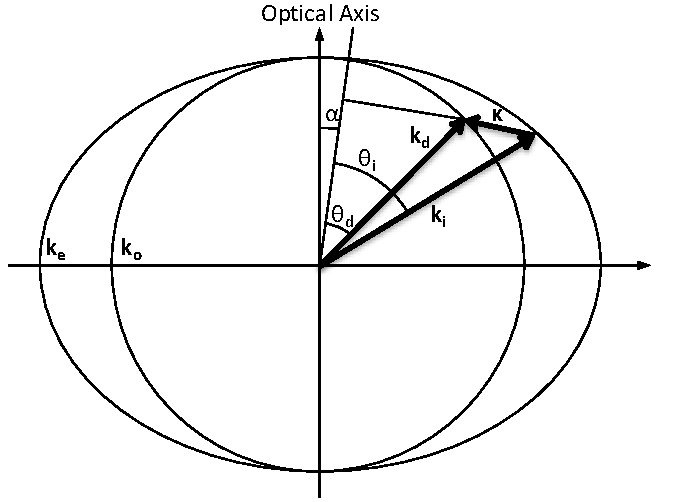
\includegraphics[width=0.7\textwidth]{./Images/3-1-AOTFWavevectorWithRefraction.pdf}
    \caption[Wave Vectors Generated by an AOTF]{The wave vectors generated by the AOTF experiment set up in \autoref{fig:3.1:AOTFExperimentalSetUp}. From the above figure $k_{e}$ and $k_{o}$ are the wave vectors of the extraordinary and ordinary axis of the AOTF crystal and can be represented as $2\pi n_{e}/\lambda$ and $2\pi n_{o}/\lambda$ respectively. The cut angel, $\alpha$, is the cut angle form the optional axis to the piezoelectric transducer.}
    \label{fig:3.1:ATOFWavevectors}
    \end{center}
\end{figure}

\begin{figure}[h!]
    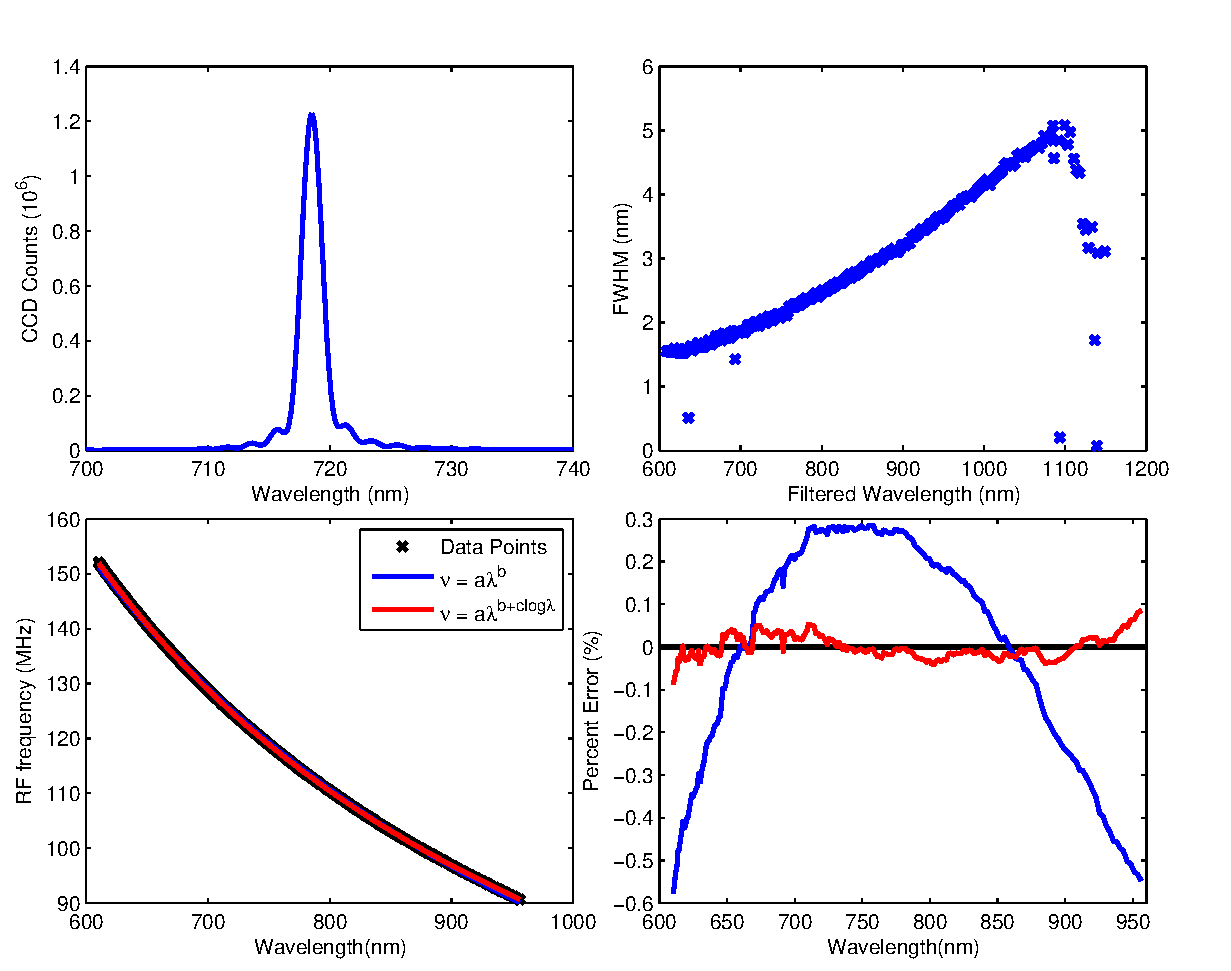
\includegraphics[width=1.0\textwidth]{./Images/3-1-AOTFCharaterization.pdf}
    \caption[Characterization Curves for the Brimrose AOTF]{Top Left: A standard image taken from the AOTF calibration experiment when the tuning frequency of the AOTF was at 124.96~MHz. Top Right: The FWHM for each of the determined wavelengths for the AOTF. It should be noted that the FWHM at 600~nm is 1.5~and as the wavelengths get longer the FWHM increases to 4.9 at 1080~nm. Bottom Left: The calibration curves for the AOTF RF versus the  diffracted wavelength which contains the data points recorded and two best fit curves. Bottom Right: The percent error with respect to the measured frequency for the two best fit curves in the previous panel. It can be noted the modified power function approximates the AOTF wavelength dependance to within 0.1\%.}
    \label{fig:3.1:AOTFCharaterization}
\end{figure}

\begin{figure}[h!]
    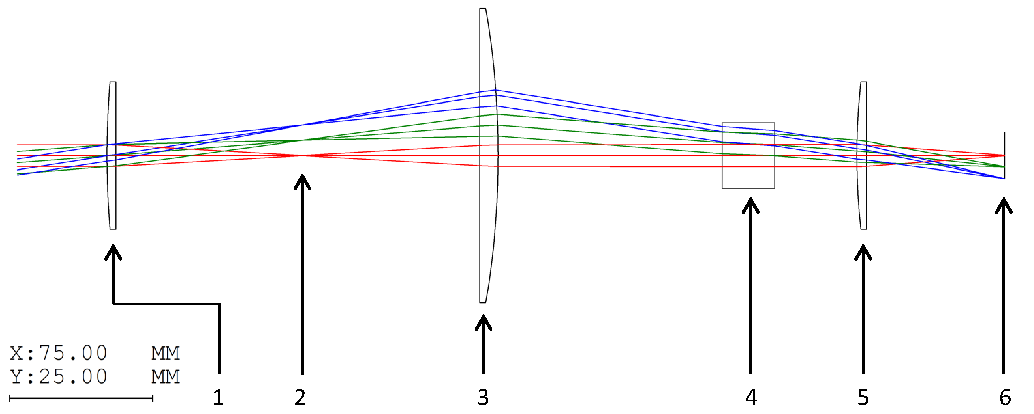
\includegraphics[width=1.0\textwidth]{./Images/3-2-TelescopicRayTracing.pdf}
    \caption[ALI Telescopic Design Prototype]{Ray Tracing diagram of the telescopic lens system simulated by Code V. The elements in the system are the following: (1) 100~mm focal length plano-convex lens. (2) Location where shutter will be located to limit stray light (3) 100~mm focal length plano-convex lens. (4) Brimrose AOTF characterized in \autoref{sec:3.1:AOTFCalibration}. (5) 75.6~mm focal length plano-convex lens. (6) Imaging plane. It should be noted that the x and y scales are not the same in this image. Also, in the lab a polarizer is added in front and behind the AOTF as well as prisms behind the AOTF.}
    \label{fig:3.2:telescopicRayTracing}
\end{figure}

\begin{figure}[h!]
    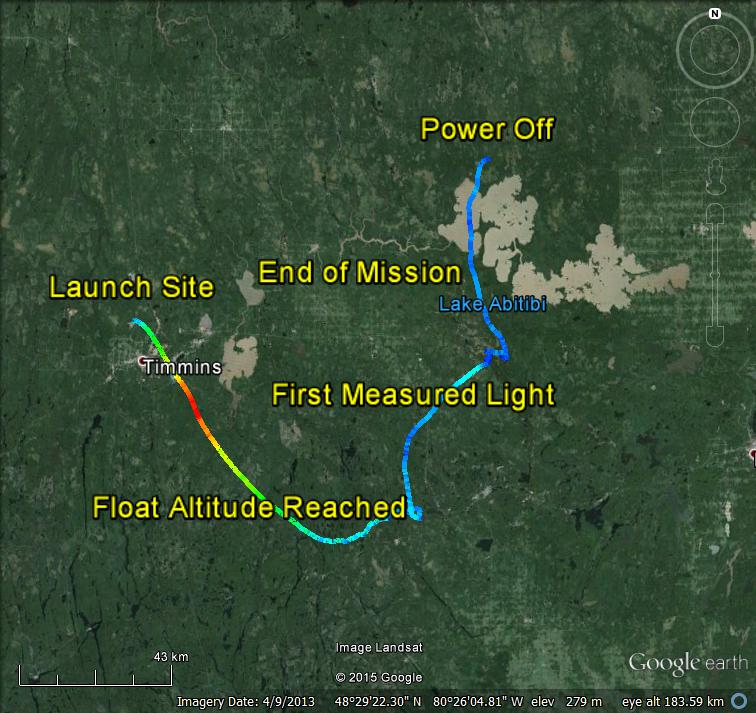
\includegraphics[width=1.0\textwidth]{./Images/5-1-AliGpsDataGoogleMaps.jpg}
    \caption[Flight Path of the Nimbus 7 Mission]{The GPS data from ALI during the Nimbus 7 mission generated via Google Earth. The colour of the line represents the absolute speed of the gondola during the mission. Important landmarks noted on the image. The end of mission represent the end of the primary aerosol mission. No GPS data was collected from ALI after the power down.}
    \label{fig:5.1:nimbus7FlightPath}
\end{figure}



\end{document} 